\documentclass[aspectratio=169,11pt]{beamer}

\usetheme{SimplePlus}

\usepackage{amsmath}
\usepackage{amssymb}
\usepackage{booktabs}
\usepackage{graphicx}
\usepackage{array}

\graphicspath{{images/lecture-1/}}

\title{S181M116 Derivatives and Alternative Investments}
\subtitle{Lecture 1: Introduction, Futures Markets, and Risk Lessons}
\author{Swapnil Singh}
\institute{Lietuvos Bankas and Kaunas University of Technology}
\date{}

\newcommand{\St}{S_T}
\newcommand{\Fzero}{F_0}
\newcommand{\Ft}{F_t}
\newcommand{\K}{K}
\newcommand{\pnl}{\mathrm{P\&L}}

\begin{document}

\begin{frame}
    \titlepage
\end{frame}

\begin{frame}{Today}
    \begin{enumerate}
        \item What derivative contracts are and why they matter.
        \item Exchange-traded versus OTC market structure.
        \item Forward, futures, and option payoffs.
        \item Futures contract design, convergence, margin, and clearing.
        \item Hedging, speculation, arbitrage, and why these labels matter.
        \item Risk-management lessons from derivatives mishaps.
    \end{enumerate}
\end{frame}

\begin{frame}{Core Message}
    \begin{block}{Derivative markets combine three layers}
        \begin{enumerate}
            \item \textbf{Contract economics:} what future cash flows are promised?
            \item \textbf{Market plumbing:} who guarantees performance, posts collateral, and settles gains/losses?
            \item \textbf{Pricing logic:} can the payoff be replicated or bounded by no-arbitrage?
        \end{enumerate}
    \end{block}

    \vspace{0.4em}
    A student who knows only the formula misses the institution.
    A student who knows only the institution misses the valuation logic.
\end{frame}

\section{Derivative Basics}

\begin{frame}{What Is a Derivative?}
    \begin{block}{Definition}
        A derivative is a contract whose value depends on an underlying variable.
    \end{block}

    \begin{itemize}
        \item The underlying can be a stock, bond, exchange rate, commodity, index, interest rate, credit event, or weather variable.
        \item The contract specifies cash flows at one or more future dates.
        \item A simple representation is
        \[
            \text{payoff at }T = g(X_T),
        \]
        where $X_T$ is the underlying variable at maturity.
    \end{itemize}
\end{frame}

\begin{frame}{Why Derivatives Matter}
    \begin{columns}[T]
        \begin{column}{0.50\textwidth}
            \begin{block}{Useful}
                \begin{itemize}
                    \item Transfer risk.
                    \item Lock in future prices.
                    \item Complete markets.
                    \item Improve price discovery.
                    \item Create tailored exposures.
                \end{itemize}
            \end{block}
        \end{column}
        \begin{column}{0.50\textwidth}
            \begin{alertblock}{Dangerous when misused}
                \begin{itemize}
                    \item Embedded leverage.
                    \item Margin and liquidity pressure.
                    \item Model error.
                    \item Counterparty exposure.
                    \item Weak governance.
                \end{itemize}
            \end{alertblock}
        \end{column}
    \end{columns}
\end{frame}

\begin{frame}{Market Size}
    \begin{center}
        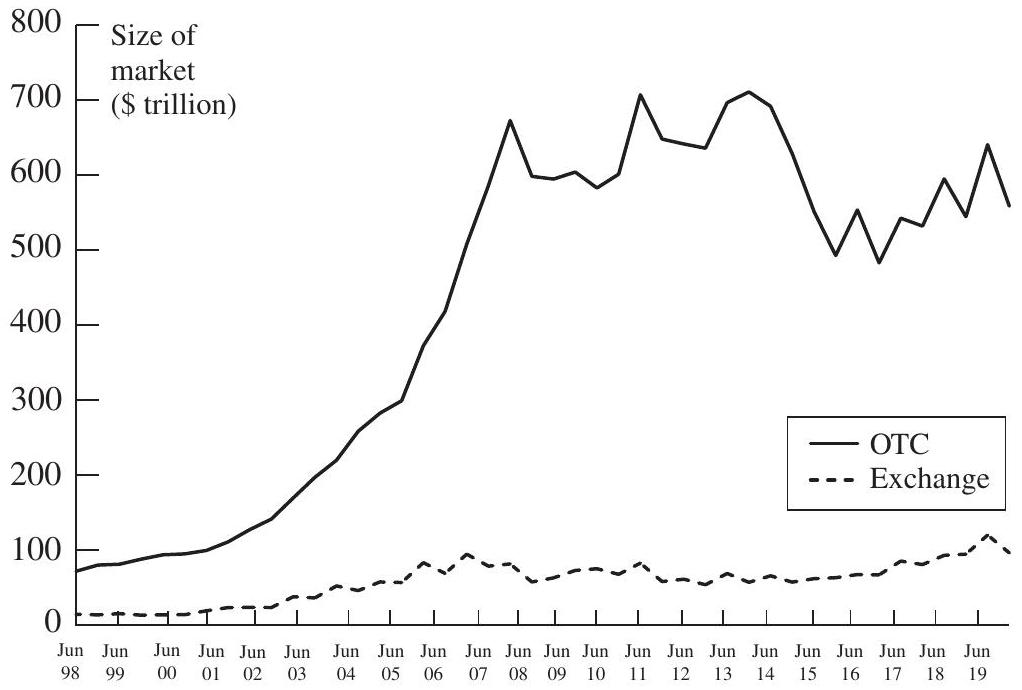
\includegraphics[width=0.82\textwidth,height=0.58\textheight,keepaspectratio]{ead832f5-1069-4974-84bd-4a1adcf0b304-027_690_1022_1578_365.jpg}
    \end{center}

    \begin{itemize}
        \item Notional measures scale, not current value-at-risk.
        \item Gross market value is smaller, but notional matters for leverage and interconnectedness.
    \end{itemize}
\end{frame}

\begin{frame}{Payoff, Profit, and Value}
    \begin{description}
        \item[Payoff] Cash flow at maturity, usually as a function of $S_T$.
        \item[Profit] Payoff minus initial cost and financing costs.
        \item[Value] Market value of the contract today.
    \end{description}

    \vspace{0.6em}
    \begin{exampleblock}{Example}
        A call option payoff may be positive at maturity, but the buyer's profit also subtracts the premium paid upfront.
    \end{exampleblock}

    \vspace{0.4em}
    We will be precise about these distinctions throughout the course.
\end{frame}

\section{Market Structure}

\begin{frame}{Exchange-Traded Derivatives}
    \begin{itemize}
        \item Contracts are standardized by the exchange.
        \item Trading is anonymous and usually electronic.
        \item The clearing house stands between buyers and sellers.
        \item Credit risk is controlled through margin, daily settlement, and default funds.
    \end{itemize}

    \begin{block}{Key idea}
        Standardization reduces customization but improves liquidity and clearing.
    \end{block}
\end{frame}

\begin{frame}{OTC Derivatives}
    \begin{itemize}
        \item OTC contracts are privately negotiated.
        \item Maturity, notional, payoff, collateral, and settlement terms can be customized.
        \item Many standardized OTC trades are now centrally cleared.
        \item Nonstandard trades can remain bilateral, governed by collateral and close-out agreements.
    \end{itemize}

    \begin{alertblock}{Trade-off}
        OTC flexibility comes with valuation, liquidity, legal, and counterparty-risk complications.
    \end{alertblock}
\end{frame}

\begin{frame}{Bilateral Clearing Versus CCP Clearing}
    \begin{center}
        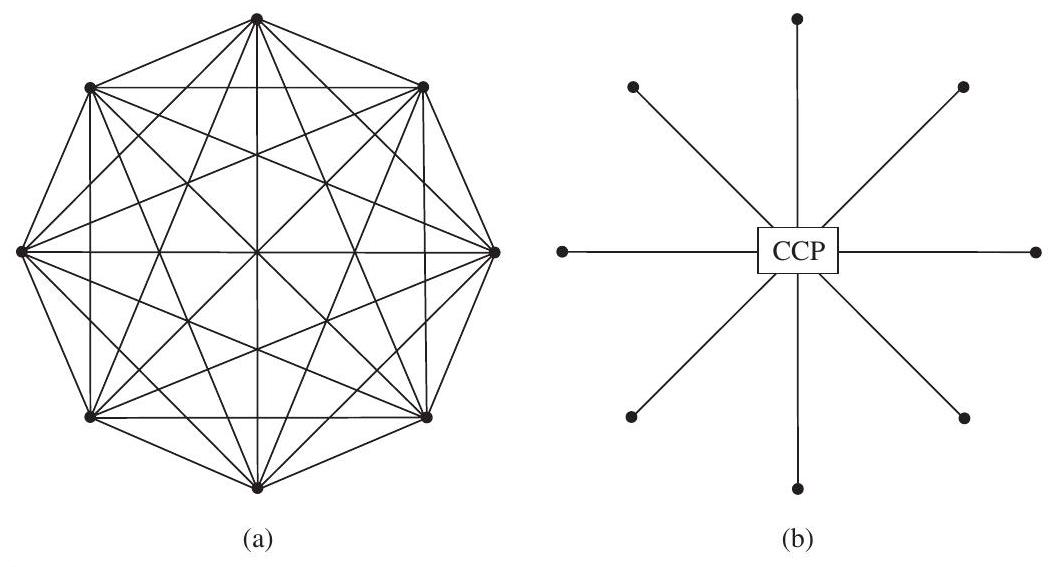
\includegraphics[width=0.86\textwidth,height=0.68\textheight,keepaspectratio]{ead832f5-1069-4974-84bd-4a1adcf0b304-057_567_1059_410_359.jpg}
    \end{center}
\end{frame}

\begin{frame}{Counterparty Risk and Systemic Risk}
    \begin{block}{Counterparty risk}
        The risk that the other side of a contract fails to perform.
    \end{block}

    \begin{block}{Systemic risk}
        The risk that one institution's failure causes losses or funding stress elsewhere in the system.
    \end{block}

    \begin{itemize}
        \item OTC networks can transmit distress.
        \item CCPs reduce bilateral exposure but concentrate risk-management responsibility.
        \item Collateral reduces credit risk but can create liquidity pressure.
    \end{itemize}
\end{frame}

\section{Forward Contracts}

\begin{frame}{Forward Contract}
    \begin{block}{Definition}
        A forward contract is an agreement to buy or sell an asset at future date $T$ for delivery price $K$.
    \end{block}

    \begin{columns}[T]
        \begin{column}{0.5\textwidth}
            \textbf{Long forward}
            \begin{itemize}
                \item Agrees to buy at $K$.
                \item Benefits when $S_T>K$.
            \end{itemize}
        \end{column}
        \begin{column}{0.5\textwidth}
            \textbf{Short forward}
            \begin{itemize}
                \item Agrees to sell at $K$.
                \item Benefits when $S_T<K$.
            \end{itemize}
        \end{column}
    \end{columns}
\end{frame}

\begin{frame}{Forward Payoffs}
    \begin{columns}[T]
        \begin{column}{0.50\textwidth}
            \centering
            Long payoff: $S_T-K$

            \vspace{0.4em}
            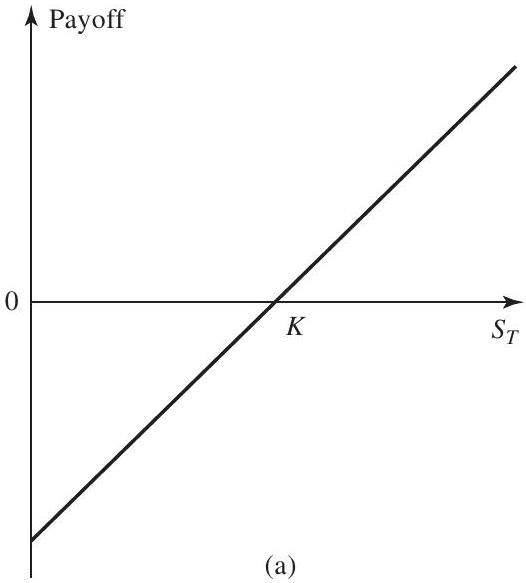
\includegraphics[width=0.70\linewidth]{ead832f5-1069-4974-84bd-4a1adcf0b304-030_583_526_380_457.jpg}
        \end{column}
        \begin{column}{0.50\textwidth}
            \centering
            Short payoff: $K-S_T$

            \vspace{0.4em}
            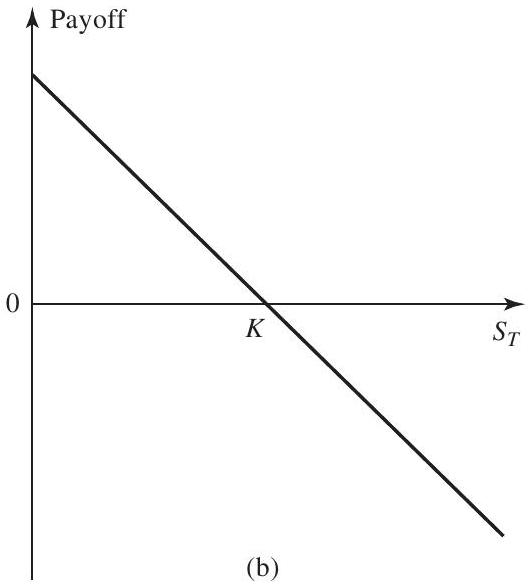
\includegraphics[width=0.70\linewidth]{ead832f5-1069-4974-84bd-4a1adcf0b304-030_585_528_378_1111.jpg}
        \end{column}
    \end{columns}
\end{frame}

\begin{frame}{Forward Hedge Example}
    A U.S. firm must pay GBP 1 million in six months.

    \begin{itemize}
        \item Six-month forward quote: USD 1.2230 per GBP.
        \item The firm enters a long GBP forward.
        \item It locks in a dollar payment of
        \[
            1{,}000{,}000 \times 1.2230 = \$1{,}223{,}000.
        \]
    \end{itemize}

    \begin{exampleblock}{If $S_T=1.3000$}
        Forward payoff is
        \[
            (1.3000-1.2230)\times 1{,}000{,}000=\$77{,}000.
        \]
    \end{exampleblock}
\end{frame}

\begin{frame}{Forward Price: First No-Arbitrage Preview}
    For a non-dividend-paying asset:
    \[
        F_0 = S_0 e^{rT}.
    \]

    \begin{block}{Why?}
        Buying the asset today and financing it must cost the same as agreeing today to buy it later.
    \end{block}

    \begin{itemize}
        \item If $F_0>S_0e^{rT}$: borrow, buy the asset, short the forward.
        \item If $F_0<S_0e^{rT}$: short the asset, invest proceeds, long the forward.
    \end{itemize}
\end{frame}

\begin{frame}{Cash-and-Carry Arbitrage}
    Suppose $S_0=60$, $r=5\%$ simple annual rate, and $T=1$.
    Then the no-arbitrage forward price is
    \[
        F_0 = 60(1.05)=63.
    \]

    \begin{alertblock}{If the quoted forward price is 67}
        \begin{enumerate}
            \item Borrow 60.
            \item Buy the asset.
            \item Short the forward at 67.
            \item At maturity, deliver asset, receive 67, repay 63.
        \end{enumerate}
        Locked-in profit: $67-63=4$.
    \end{alertblock}
\end{frame}

\section{Futures Markets}

\begin{frame}{Futures Contract}
    A futures contract is similar to a forward contract economically, but not institutionally.

    \begin{table}
        \centering
        \begin{tabular}{lll}
            \toprule
            Feature & Forward & Futures \\
            \midrule
            Venue & OTC & Exchange \\
            Terms & Customized & Standardized \\
            Counterparty & Bilateral/CCP & Clearing house \\
            Settlement & Usually maturity & Daily \\
            Initial cash flow & Usually none & Margin \\
            \bottomrule
        \end{tabular}
    \end{table}
\end{frame}

\begin{frame}{Contract Specification}
    A futures exchange must define:
    \begin{itemize}
        \item underlying asset and acceptable grades;
        \item contract size;
        \item delivery months;
        \item delivery location and delivery process;
        \item price quotation convention;
        \item tick size;
        \item price limits and position limits.
    \end{itemize}

    \begin{block}{Why so much detail?}
        Standardization makes the contract tradable by many participants who do not know each other.
    \end{block}
\end{frame}

\begin{frame}{Convergence}
    As delivery approaches, the futures price converges to the spot price.

    \begin{center}
        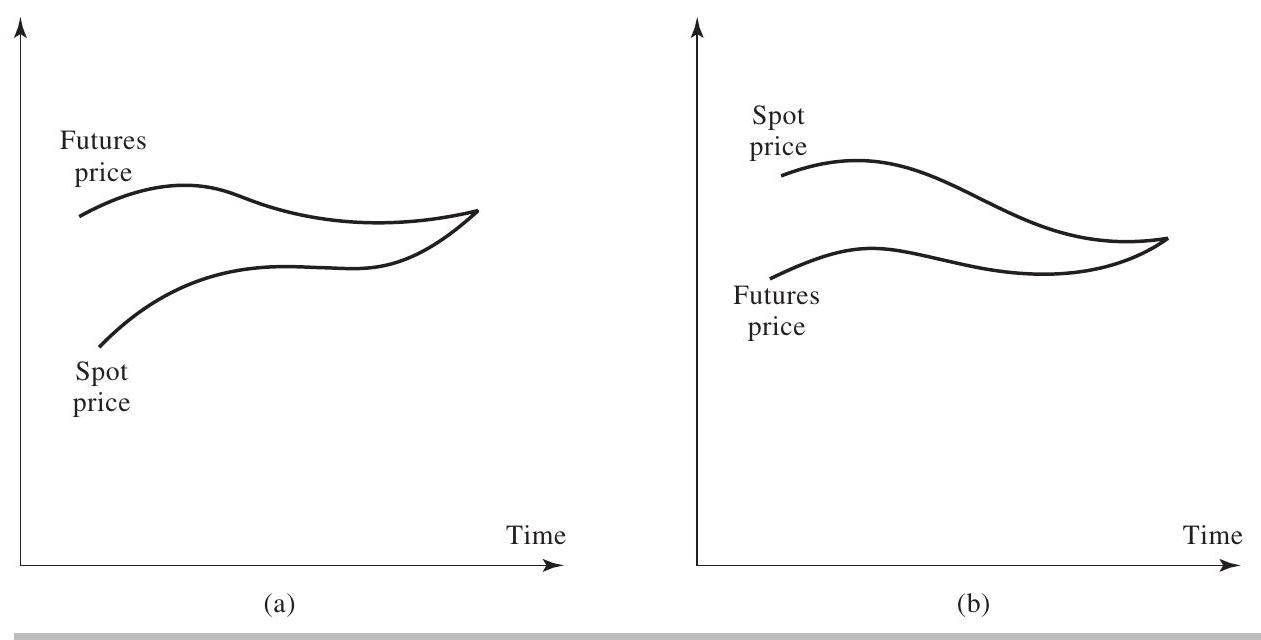
\includegraphics[width=0.70\textwidth,height=0.50\textheight,keepaspectratio]{ead832f5-1069-4974-84bd-4a1adcf0b304-051_640_1261_384_361.jpg}
    \end{center}

    \begin{block}{Anchor}
        Even when delivery is rare, the possibility of delivery ties the futures market to the cash market.
    \end{block}
\end{frame}

\begin{frame}{Margin Is Collateral}
    \begin{block}{Margin is not the price of the futures contract}
        It is collateral posted to protect the clearing system against default.
    \end{block}

    \begin{itemize}
        \item \textbf{Initial margin:} amount deposited when the position is opened.
        \item \textbf{Maintenance margin:} minimum acceptable balance.
        \item \textbf{Margin call:} request to restore the account after losses.
        \item \textbf{Variation margin:} daily settlement of gains and losses.
    \end{itemize}
\end{frame}

\begin{frame}{Daily Settlement}
    Let $N$ be the number of contracts and $Q$ the contract size.

    \begin{block}{Long futures daily P\&L}
        \[
            \pnl_t = NQ(F_t-F_{t-1}).
        \]
    \end{block}

    \begin{block}{Short futures daily P\&L}
        \[
            \pnl_t^{short}=NQ(F_{t-1}-F_t).
        \]
    \end{block}

    Futures gains and losses are realized daily, not merely at maturity.
\end{frame}

\begin{frame}{Margin Example}
    A trader is long two gold futures contracts.
    Each contract is for 100 ounces.

    \begin{itemize}
        \item Total exposure: $2\times 100=200$ ounces.
        \item Yesterday's settlement: $F_{t-1}=1{,}750$.
        \item Today's settlement: $F_t=1{,}741$.
    \end{itemize}

    \[
        \pnl_t = 200(1{,}741-1{,}750)=-1{,}800.
    \]

    \begin{alertblock}{Interpretation}
        The long loses USD 1,800 today. The short gains USD 1,800 today.
    \end{alertblock}
\end{frame}

\begin{frame}{Why Futures Can Create Liquidity Risk}
    \begin{itemize}
        \item Daily settlement reduces credit risk to the clearing house.
        \item But it forces losing traders to fund losses immediately.
        \item A trader can be correct about the final price and still fail because interim margin calls are too large.
    \end{itemize}

    \begin{alertblock}{Risk-management lesson}
        Mark-to-market discipline controls default risk but can transform market risk into funding pressure.
    \end{alertblock}
\end{frame}

\section{Options}

\begin{frame}{Options}
    \begin{block}{Call option}
        Gives the holder the right, but not the obligation, to buy the underlying at strike price $K$.
    \end{block}

    \begin{block}{Put option}
        Gives the holder the right, but not the obligation, to sell the underlying at strike price $K$.
    \end{block}

    The option buyer pays a premium because the payoff is one-sided.
\end{frame}

\begin{frame}{Option Payoffs}
    \[
        \text{Call payoff} = \max(S_T-K,0)=(S_T-K)^+
    \]
    \[
        \text{Put payoff} = \max(K-S_T,0)=(K-S_T)^+
    \]

    \begin{itemize}
        \item Forward payoff is linear.
        \item Option payoff is kinked and convex.
        \item Convexity is why option pricing requires more machinery than forward pricing.
    \end{itemize}
\end{frame}

\begin{frame}{Option Profit Is Not Option Payoff}
    \begin{center}
        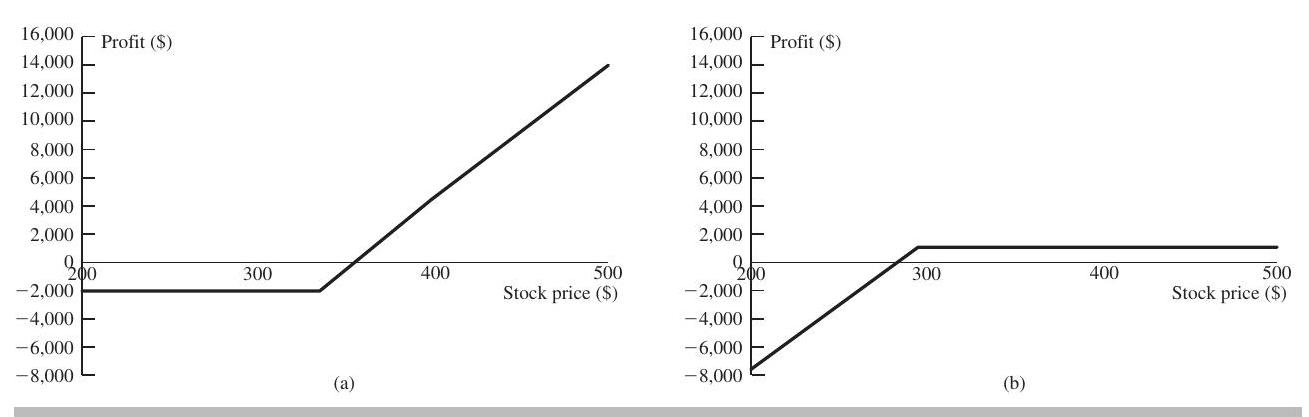
\includegraphics[width=0.76\textwidth,height=0.58\textheight,keepaspectratio]{ead832f5-1069-4974-84bd-4a1adcf0b304-033_417_1309_425_361.jpg}
    \end{center}

    \begin{block}{Premium matters}
        The buyer's payoff can be positive while profit is still negative if the payoff does not exceed the premium.
    \end{block}
\end{frame}

\begin{frame}{American Versus European Options}
    \begin{columns}[T]
        \begin{column}{0.50\textwidth}
            \begin{block}{European}
                Exercise only at maturity.
            \end{block}
        \end{column}
        \begin{column}{0.50\textwidth}
            \begin{block}{American}
                Exercise any time up to maturity.
            \end{block}
        \end{column}
    \end{columns}

    \vspace{1em}
    Since American options give more flexibility,
    \[
        C_A \geq C_E,\qquad P_A \geq P_E.
    \]
\end{frame}

\section{Users of Derivatives}

\begin{frame}{Hedgers}
    A hedger uses derivatives to reduce an existing exposure.

    \begin{center}
        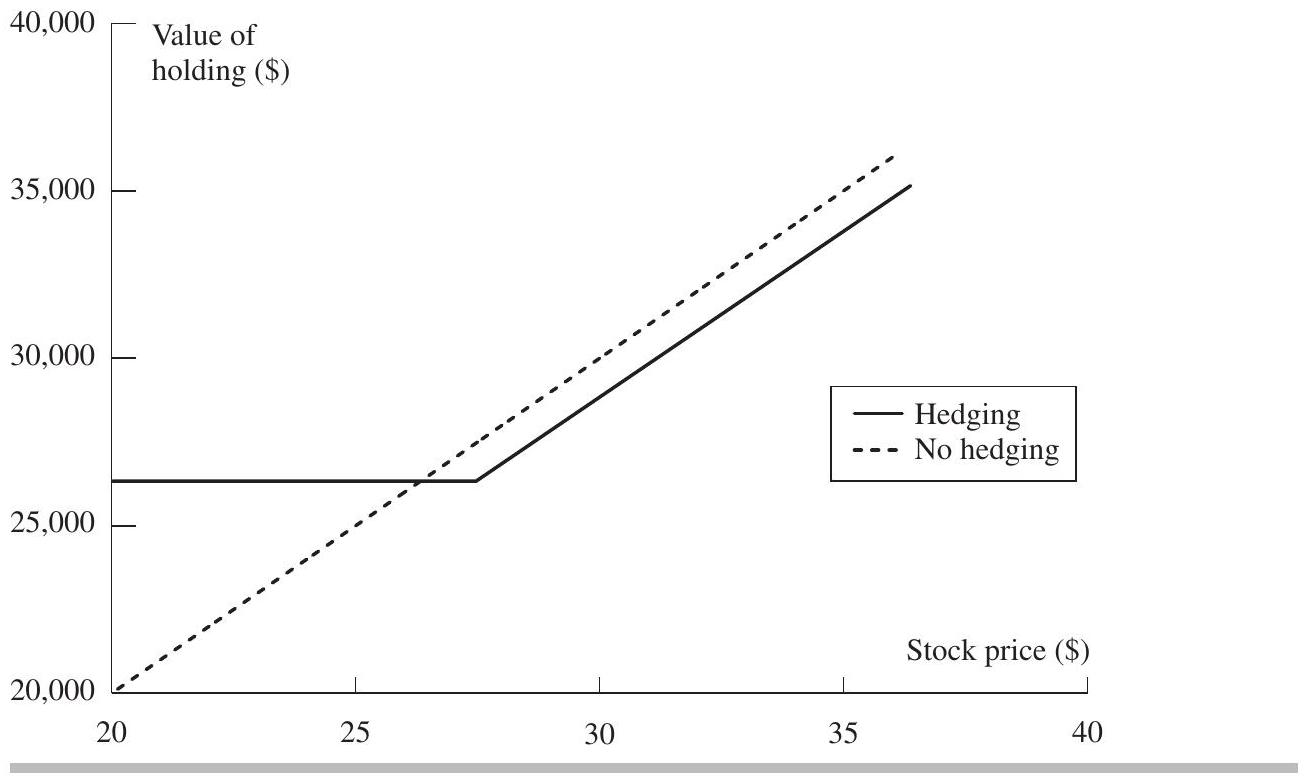
\includegraphics[width=0.76\textwidth,height=0.56\textheight,keepaspectratio]{ead832f5-1069-4974-84bd-4a1adcf0b304-035_782_1309_1527_365.jpg}
    \end{center}

    \begin{block}{Evaluation}
        Do not judge the derivative leg alone. Judge the combined position.
    \end{block}
\end{frame}

\begin{frame}{Speculators}
    A speculator uses derivatives to take a view on market direction, volatility, spreads, or timing.

    \begin{itemize}
        \item Futures allow large notional exposure with margin rather than full purchase price.
        \item Options allow directional views with limited downside for buyers.
        \item Leverage makes both gains and losses arrive faster.
    \end{itemize}

    \begin{center}
        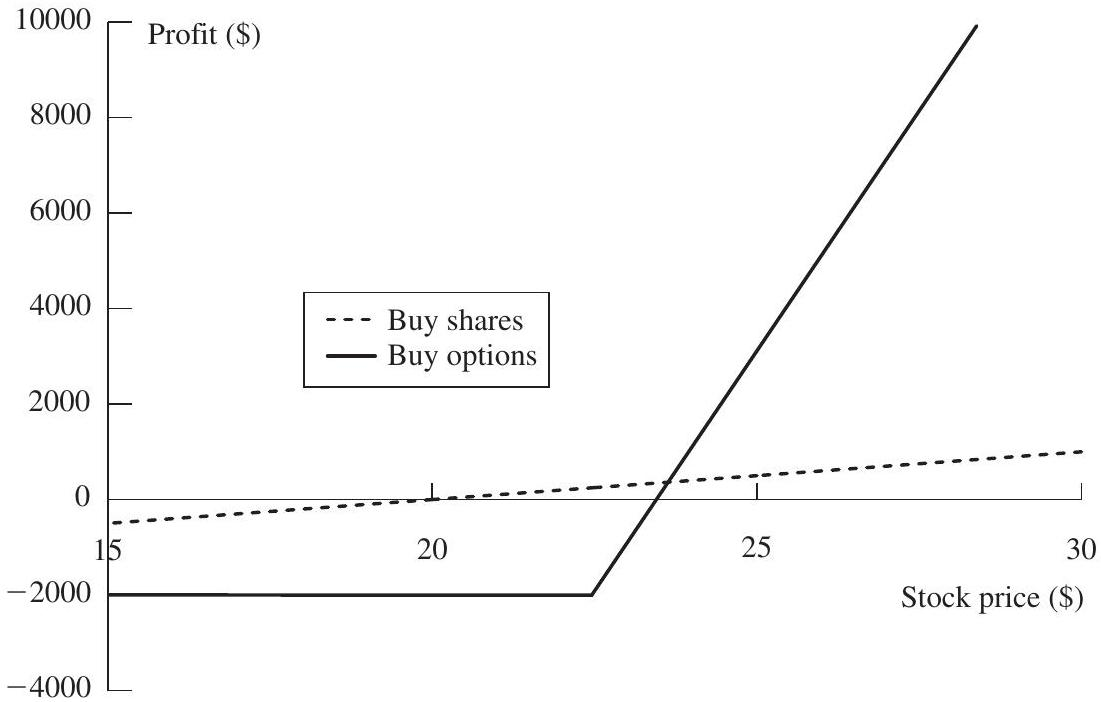
\includegraphics[width=0.60\textwidth,height=0.34\textheight,keepaspectratio]{ead832f5-1069-4974-84bd-4a1adcf0b304-038_702_1101_398_458.jpg}
    \end{center}
\end{frame}

\begin{frame}{Arbitrageurs}
    An arbitrageur tries to lock in a profit by exploiting inconsistent prices.

    \begin{block}{True arbitrage}
        No net investment, no risk of loss, positive profit in at least one state.
    \end{block}

    \begin{alertblock}{Convergence trading is not true arbitrage}
        Many trades called arbitrage can lose money before prices converge. They are exposed to funding, liquidity, and model risk.
    \end{alertblock}
\end{frame}

\section{Risk Lessons}

\begin{frame}{Why Study Mishaps in Lecture 1?}
    \begin{itemize}
        \item Derivatives losses are rarely caused by equations alone.
        \item They usually combine leverage, weak controls, bad incentives, poor liquidity, and misunderstood models.
        \item The same instrument can be a hedge in one balance sheet and a speculative weapon in another.
    \end{itemize}

    \begin{block}{Course discipline}
        Every pricing formula must be paired with its assumptions and its risk-management limits.
    \end{block}
\end{frame}

\begin{frame}{Common Failure Modes}
    \begin{enumerate}
        \item Market moves against the position.
        \item Position size is too large relative to capital.
        \item Margin calls arrive before the strategy pays off.
        \item Model prices or hedge ratios are wrong.
        \item Traders can hide or misreport risk.
        \item Risk limits are ignored after profitable breaches.
        \item Incentives reward short-term gains and hide tail losses.
    \end{enumerate}
\end{frame}

\begin{frame}{Risk Limits}
    A good risk limit answers four questions:

    \begin{enumerate}
        \item What exposure is being limited?
        \item How is the exposure measured?
        \item Who is notified when the limit is breached?
        \item What action follows the breach?
    \end{enumerate}

    \begin{exampleblock}{Examples}
        Notional limits, VaR limits, stress-loss limits, Greek limits, stop-loss limits, maturity limits, counterparty limits, liquidity limits.
    \end{exampleblock}
\end{frame}

\begin{frame}{Front, Middle, and Back Office}
    \begin{description}
        \item[Front office] Trades, manages client relationships, and generates revenue.
        \item[Middle office] Measures risk, validates prices, monitors limits, and challenges assumptions.
        \item[Back office] Confirms trades, settles cash flows, reconciles positions, and maintains records.
    \end{description}

    \begin{alertblock}{Control principle}
        The person taking risk should not be the only person measuring, confirming, and reporting that risk.
    \end{alertblock}
\end{frame}

\begin{frame}{Model Risk}
    Models are useful simplifications, not reality.

    \begin{itemize}
        \item wrong model for the product;
        \item wrong parameters;
        \item ignored liquidity and transaction costs;
        \item unstable correlations in stress periods;
        \item untested extrapolation;
        \item users who do not understand assumptions.
    \end{itemize}

    \begin{block}{Rule}
        A formula without assumptions is not knowledge.
    \end{block}
\end{frame}

\section{Wrap-Up}

\begin{frame}{What You Should Know After Lecture 1}
    \begin{itemize}
        \item Derivatives are contracts with payoffs linked to underlying variables.
        \item Exchange and OTC markets solve different problems.
        \item Forwards create binding linear exposure.
        \item Futures add standardization, clearing, margin, and daily settlement.
        \item Options give rights rather than obligations and therefore require premiums.
        \item Hedging, speculation, arbitrage, and convergence trading are different activities.
        \item Risk management is institutional, not just mathematical.
    \end{itemize}
\end{frame}

\begin{frame}{Practice Before Next Class}
    \begin{enumerate}
        \item Draw long and short forward payoff diagrams.
        \item Compute the no-arbitrage forward price for a non-dividend-paying stock.
        \item Compute daily futures P\&L for long and short positions.
        \item Explain why margin is collateral rather than purchase price.
        \item Write call and put payoffs using positive-part notation.
        \item Identify whether a trade is hedging, speculation, arbitrage, or convergence trading.
        \item Pick one derivatives mishap and identify the risk-management failures.
    \end{enumerate}
\end{frame}

\begin{frame}
    \centering
    \Large Next class: hedging with futures and forward/futures prices.
\end{frame}

\end{document}
